\documentclass{article}
\usepackage{graphicx}
\graphicspath{{images/}}

\title{
    User Manual\\
    \begin{large}
        \textit{Golf Course Mapper}
    \end{large}
}
\date{
    \begin{small}
        \today
    \end{small}
}
\author{
    Team Recursive Recursion \\
    Retro Rabbit
}

\begin{document}
    %===========================================================================
    % TITLE
    %===========================================================================
    \pagenumbering{gobble}
    \maketitle
    \newpage

    %===========================================================================
    % DOCUMENT
    %===========================================================================
    \pagenumbering{arabic}

    
    
	\section{System Overview}    
	\paragraph{}
	The project will allow golf course owners/managers to draw their golf course using the provided web application. While drawing the golf course, details about the map can be added, such as locations of the hole, green, fairway, or any obstacles and hazardous areas.
Golf players will be able to view the map via their Android phones, enabling them to have a hands-on digital map with details of the course. This will allow the user to plan their shots better and more strategically.


	\section{System Configuration}
	 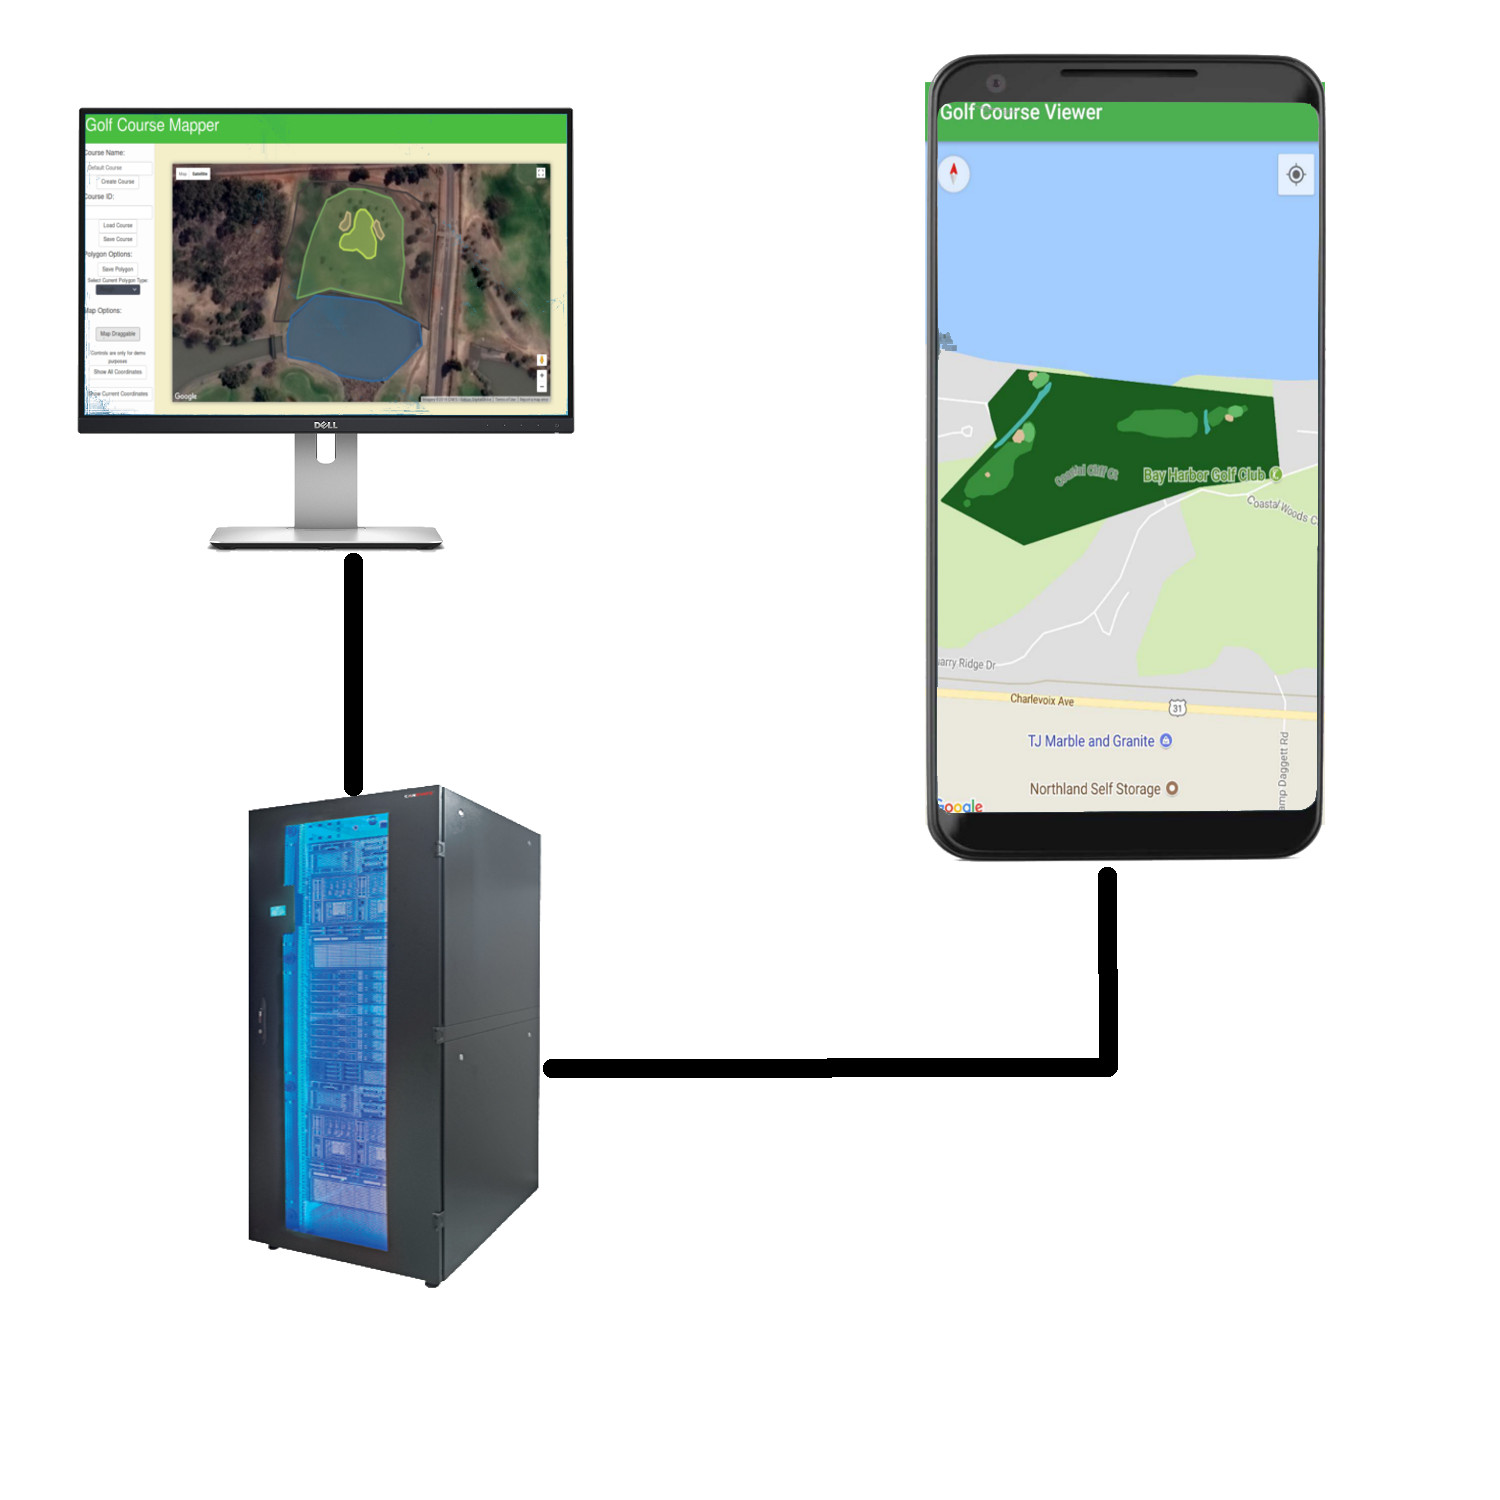
\includegraphics[scale=0.25]{sys-conf-diagram.jpg}
	\paragraph{•}
	  The web application and the mobile application connects to the server to retrieve data. An Internet connection is needed to load the map on both the web application and mobile application.
	
	\section{Getting Started}
	\paragraph{•}
	
	Web Application: To access the web application go to the URL (http://localhost:5000/home). There is no authentication needed to access the web application.
	
	Mobile Application: To access the mobile application press on the application on a mobile device.
	\section{Using the System}
    \subsection{Web Application}
    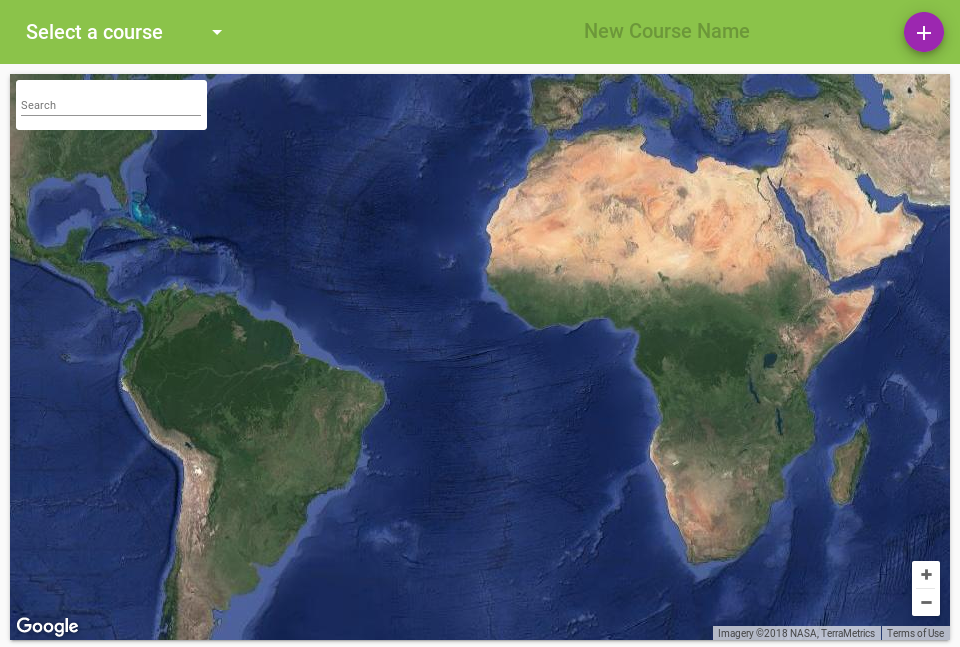
\includegraphics[scale=0.25]{map}
    \paragraph{•}
    Figure 1.
    
    \subsubsection{Create Course}
    \paragraph{•}
    Type in the name of the desired golf course to create the course as shown in Figure 1. After a appropriate name has been chosen, click on the "Create Course" button. The course will now be created with the chosen name.
    
    \subsubsection{Save Course} 
    \paragraph{}
    After changes has been been to the current course,click on the "Save Course" button to save the changes made.
    
    
    \subsubsection{Load Course}
    \paragraph{}
    To load a course type in the name of the course that you want to load, in the "Course ID" edit box. Click on the "Load Course" button. The loaded course will now be shown. See Figure 1 for reference.
    
    \subsubsection{Polygon}
    
    \paragraph{}
    To create a polygon click on the map to create a dot (vertex). By clicking multiple times on the map the polygon will be constructed. When the desired polygon is completed click on the "Save Polygon" button, as indicated in Figure 1. The polygon will now become inactive and cannot be edited.
    
    \subsubsection{Polygon Types}

    \paragraph{}
    To change the terrain type click on the polygon type drop down menu. Choose the desired terrain option. The polygon will be updated accordingly.
    
    \subsubsection{Map Controls}
    
    \paragraph{Map Draggable}
    Click on the "Map Draggable" button. The map will now stay in the same position making the course mapping easier. To revert back to make the map draggable click on the "Map Draggable" again.
    \paragraph{Reset Map}
    Click on the "Reset Map" button to reset the map to the original state.

	\subsection{Mobile Application}
	    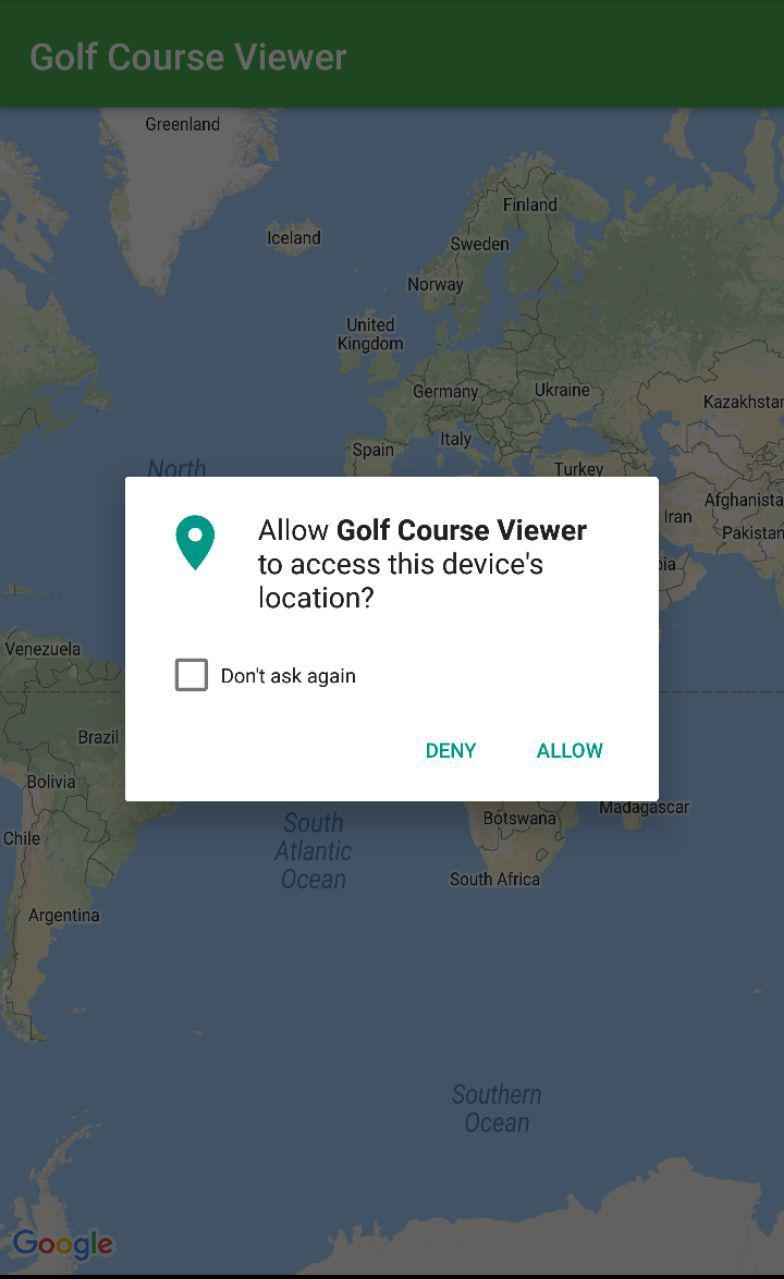
\includegraphics[scale=0.2]{mobileapp-permissions.jpg}
	\subsubsection{Allow Permissions}
	
	\paragraph{•}
	When starting the application, a message will pop up to ask for permissions to use location services. Press "Allow" to allow location services to be used.
	
	\subsubsection{View Course}
	    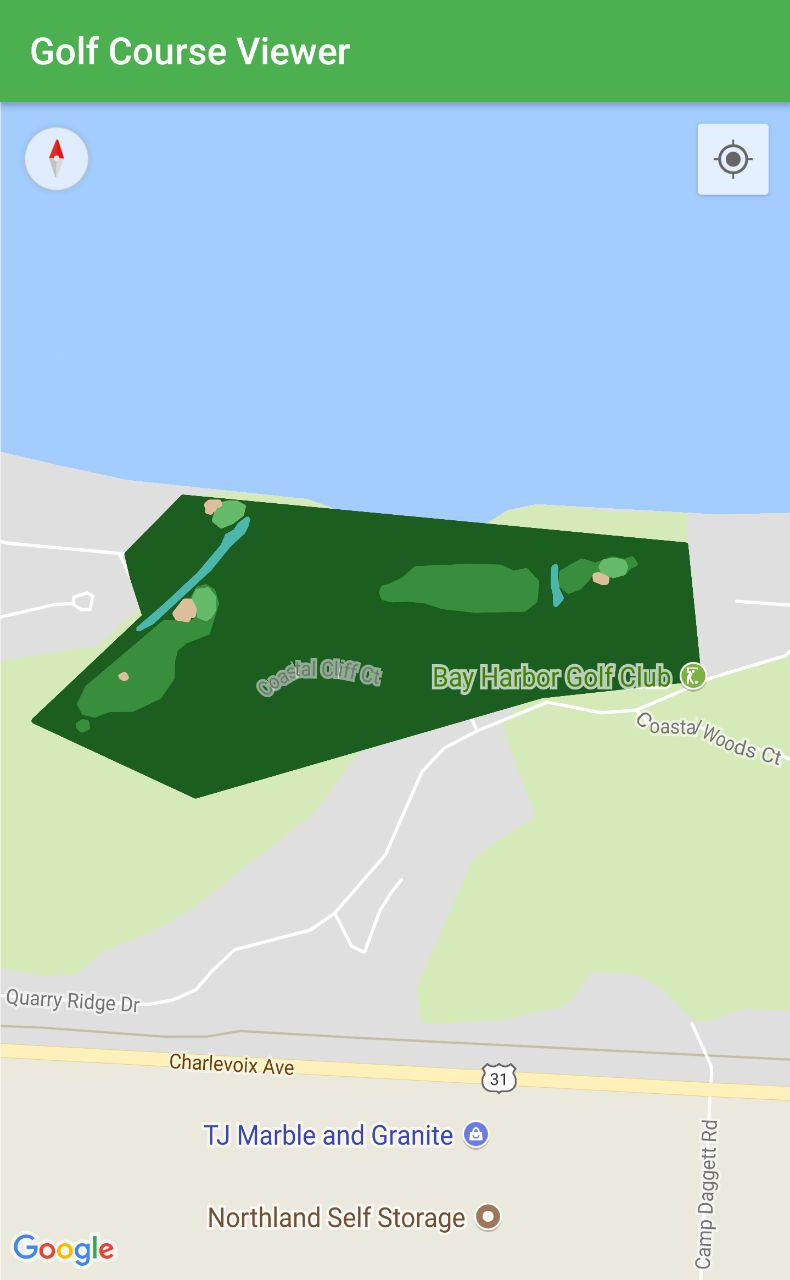
\includegraphics[scale=0.2]{mobilemap.jpg}
	
	\paragraph{•}
	Move around by touching and zoom by pinching the screen. Move to the location of gold course created to view the course.
	
	
\end{document}